%%%%%%%%%%%%%%%%%%%%%%%%%%%%%%%%%%%%%%%%%%%%%%%%%%%%%%%
% A template for Wiley article submissions.
% Developed by Overleaf. 
%
% Please note that whilst this template provides a 
% preview of the typeset manuscript for submission, it 
% will not necessarily be the final publication layout.
%
% Usage notes:
% The "blind" option will make anonymous all author, affiliation, correspondence and funding information.
% Use "num-refs" option for numerical citation and references style.
% Use "alpha-refs" option for author-year citation and references style.
\PassOptionsToPackage{author-year,initials,nobysame}{amsrefs}
\documentclass[ams-refs]{wiley-article}
% \documentclass[blind,ams-refs]{wiley-article}

% Add additional packages here if required
\usepackage{siunitx}
\usepackage{verbatim}

% Update article type if known
\papertype{Original Article}
% Include section in journal if known, otherwise delete
\paperfield{Journal Section}

\title{Presence impacts spatial exploration behavior in large scale VR}

% List abbreviations here, if any. Please note that it is preferred that abbreviations be defined at the first instance they appear in the text, rather than creating an abbreviations list.
%\abbrevs{ABC, a black cat; DEF, doesn't ever fret; GHI, goes home immediately.}

% Include full author names and degrees, when required by the journal.
% Use the \authfn to add symbols for additional footnotes and present addresses, if any. Usually start with 1 for notes about author contributions; then continuing with 2 etc if any author has a different present address.
\author[1\authfn{1}]{Lukas Gehrke}
%\author[1]{Sezen Akman}
\author[1,2,3]{Klaus Gramann PhD}

%\contrib[\authfn{1}]{Equally contributing authors.}

% Include full affiliation details for all authors
\affil[1]{Department of Biopsychology and Neuroergonomics, Institute of Psychology and Ergonomics, TU Berlin, Berlin, Berlin, 10623, Germany}
\affil[2]{Center for Advanced Neurological Engineering, University of California San Diego, San Diego, California, 92093, USA}
\affil[3]{School of Software, University of Technology Sydney, Sydney, New South Wales, 2007, Australia}
\corraddress{KWT-1 Department of Biopsychology and Neuroergonomics, Fasanenstr. 1, 10632 Berlin, Berlin, Germany}
\corremail{info@lukasgehrke.com}

\presentadd[\authfn{1}]{KWT-1 Department of Biopsychology and Neuroergonomics, Fasanenstr. 1, 10632 Berlin, Berlin, Germany}

\fundinginfo{This research was supported by a grant from the German Federal Ministry of Education and Research (01GQ1511) to KG}



% Include the name of the author that should appear in the running header
\runningauthor{Lukas Gehrke et al.}

\begin{document}

\maketitle
% must be between 150 and 250, so aiming for 200!
\begin{abstract}
The use of head-mounted virtual reality (VR) to induce presence in a computer simulated world has proven to significantly increase the ecological validity of this medium. In VR, illusions of various kinds (place illusion, plausibility illusion, etc.) occur at the same time for the user to feel present. Most prominently, the embodiment illusion has proven to elicit 'realistic' behavioral as well as physiological responses, when a strong emotional stimulus such as virtual hurting of an embodied rubber hand is provided. Yet, to be able to employ VR and claim ecological validity for less emotional stimuli, the level of presence must be accounted for. We show that the level of presence impacts free spatial exploration behavior in a large scale VR navigation paradigm. Here, we investigate the impact of an established presence metric on ongoing motor behavior demonstrating an analysis framework with a high spatial resolution. We observed participants with higher presence to stay closer to the walls while exploring invisible mazes. Ultimately, we link presence to individual differences in video game experience, sex, and spatial perspective taking abilities, confirming that user characteristics are a defining part of the presence construct.
\end{abstract}
% in the end use hemingway app (http://www.hemingwayapp.com) to increase readability
% Word count is 194:

\section{Introduction}
Novel immersive paradigms in the behavioral cognitive sciences as well as neurosciences make use of illusions to subject participants to controlled, yet stimulus rich experiences in head-mounted virtual reality (VR). 

VR paradigms 

Depending on the effectiveness of the illusions and whether multiple illusions work in congruence, participants experience feeling present in VR. With all modern virtual reality headsets providing precise motion capture, synchronized data collection is easily accomplished and allows to address rich, natural behavior. Assuming that experiencing presence equals treating what you perceive as a part of the reality you are currently in, many researchers have argued for an increase in ecological validity employing VR in their research \cite{Bohil2011, Parsons2015, Parsons2017}. The assumption hence is that participants under the influence of VR illusions experience presence and therefore behave 'realistically' or with more ecologically validity.

\begin{figure}[t]
\centering
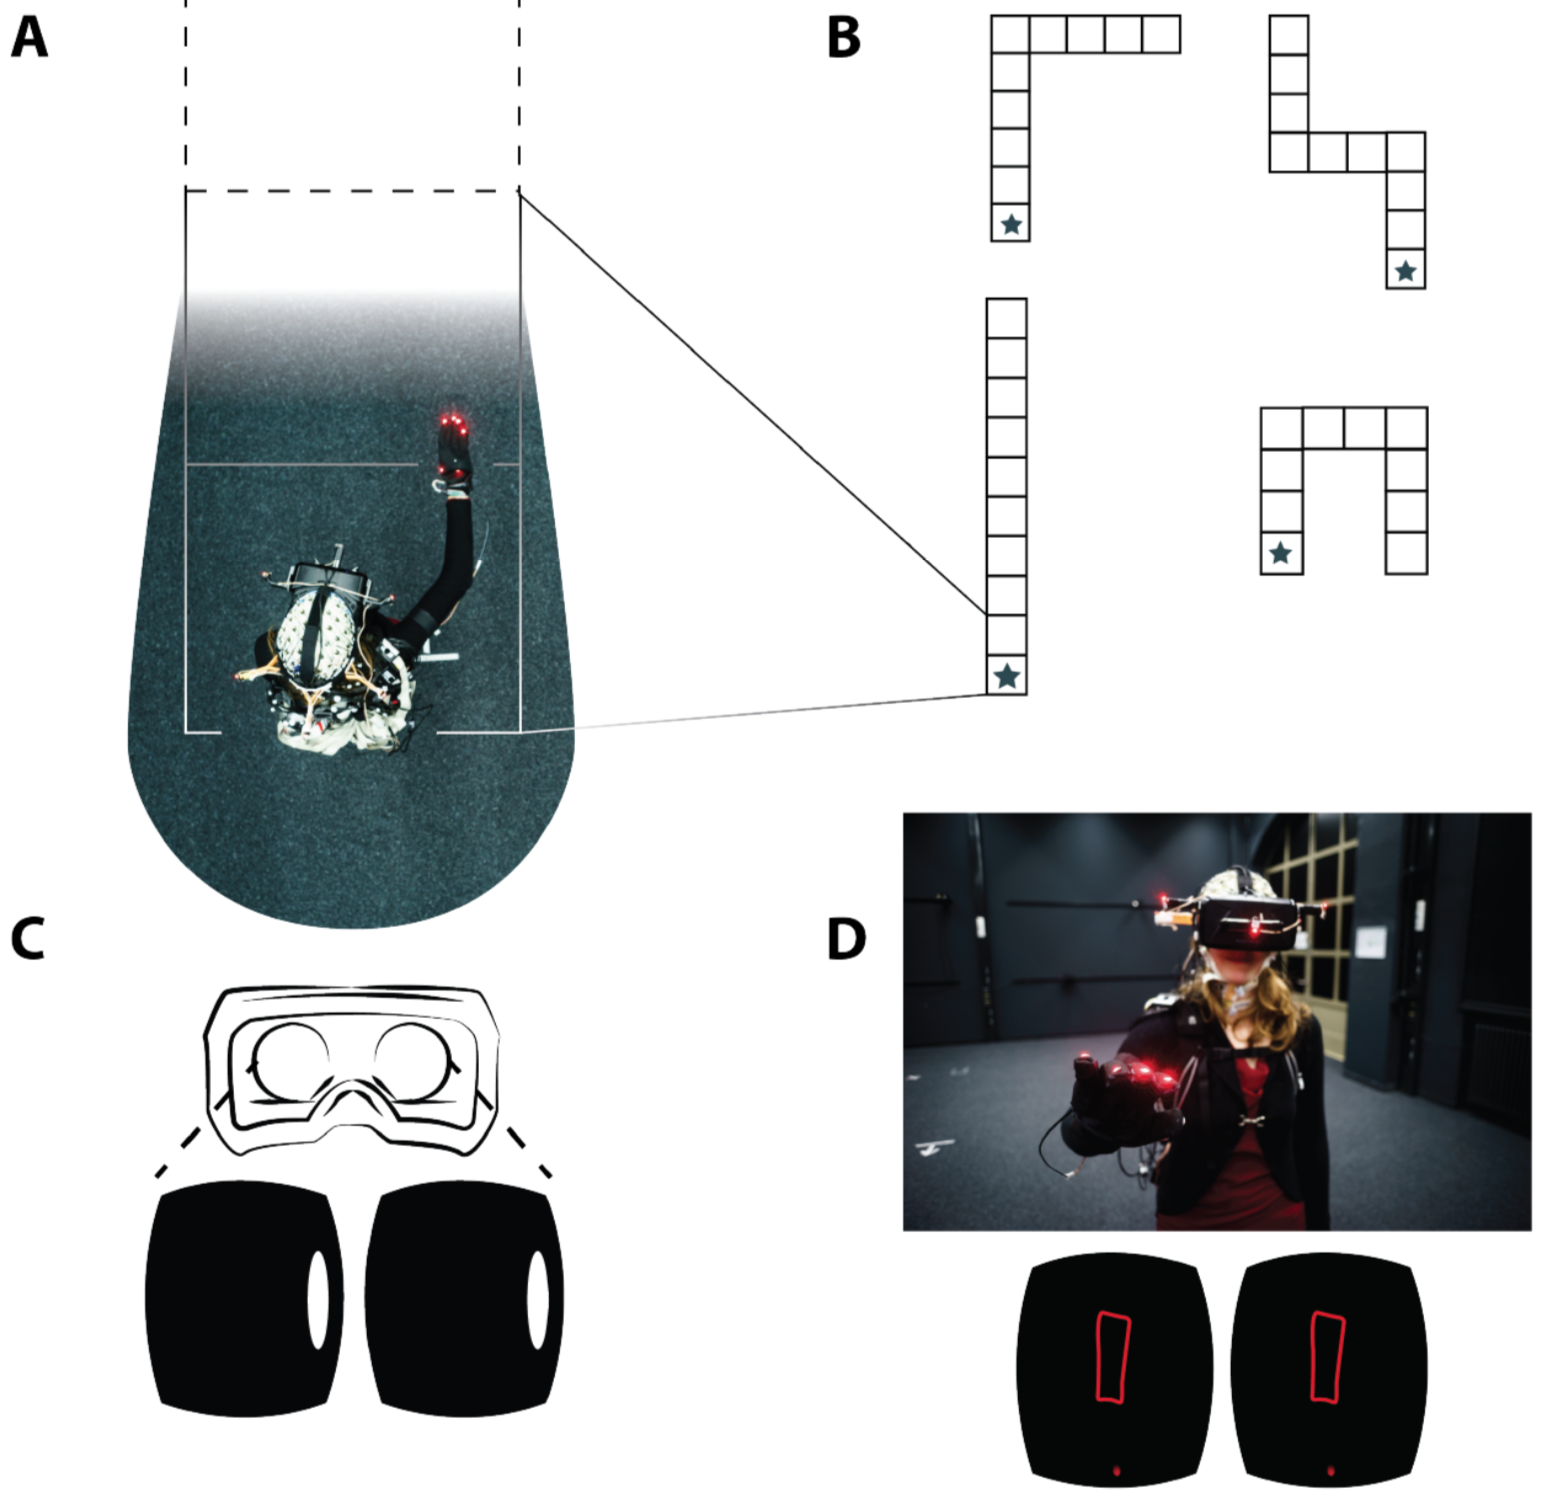
\includegraphics[width=\linewidth]{IMT_Task.png}
\vspace{0pt}
\caption{Invisible Maze Task, \textbf{A} Participant from a bird’s eye view. \textbf{B} Participants are instructed to explore four different mazes and return to the start. \textbf{C} First-person view in binocular ""VR optics"" of a wall touch. \textbf{D} Top: Participants draw a top-down view of the explored maze. Participant is equipped with 160 channels wireless EEG, head-mounted virtual reality goggles and LEDs for motion capture. Bottom: drawn sketch map. Find a detailed description in~\cite{Gehrke2018}}
\label{imt_task}
\end{figure}

% Next Paragraph: Do people behave differently in VR? And if so, does it depend on the level of experienced presence?
However, fewer studies have investigated the impact of the effectiveness of VR illusions on rich behavioral, psychometric and bio-physiological parameters. Here, the bulk of the literature focuses on (A) emotionally charged stimulus material or (B) embodiment illusions.

Considering (A), Diemer et al. provide a thorough overview of the intricate interplay between presence and reactions to emotionally charged stimulation in VR \cite{Diemer2015}. The authors observed a consistently reported link between presence and the emotional experience in VR. They argue, that by varying degrees of arousal, presence impacts psychological as well as physiological responses.

Considering (B), we highlight one relevant aspect from the rich literature on the effects of full-body embodiment into avatars \cite{Maister2015}. The proteus effect characterizes behavioral perturbations depending on avatar body attributes. Yee et al. showed that participants being immersed into an 'attractive' avatar moved closer into the interpersonal space of another person \cite{Yee2007}. Further, Banakou et al. demonstrated that within participants, the sizes of objects were overestimated while embodied into a child body compared to a non-embodied baseline \cite{Banakou2013}.
These examples illustrate that the level of experienced presence, induced through embodiment illusions, directly impacts mental representation of the surroundings and respectively the motor behavior.
\subsection{Stationary and true mobile spatial navigation in VR}

Modern virtual reality headsets provide precise motion capture and conversely allow to render a wide variety of motion illusions useful for research in spatial navigation. Using lightweight electrical (Electroencephalogram, EEG) or optical (functional near infrared spectroscopy, fNIRS) sensors concurrently, it is now feasible to digitize brain signals along with spatial location. However, different systems impose different requirements on the participants. Those technical requirements may in turn affect participants experiences, such as feeling present, in VR. \cite{} % todo effect of wires on presence
We consider a minimum of three different levels of continuous self-motion perception in head-mounted VR in the evolution from constrained stationary to unconstrained freely movements. On the first level we locate perceiving illusory motion, i.e. vection, induced through flow signals. Such flow signals can be sensible by a number of different senses, e.g. optical flow by the visual sense or wind flowing over the skin. Vection can be induced in completely immobile participants and is hence compatible with a great number of brain imaging technology that require participants to remain stationary, i.e. fMRI and MEG. The strength of the vection illusion can be significantly increased by minimal physical motion cueing \cite{}. %Riecke/Cruiff motion cueing \cite{} %Riecke arbeiten
Such physical motion cues briefly trigger the vestibular and proprioceptive sensing systems in addition to the senses perceiving flow signals. Interestingly, such cues can be delivered without physically moving the body but rather by, e.g. galvanic vestibular stimulation \cite{} % e.g. if gvs
Here lies the transition to the second level of self-motion perception in VR. Perceiving a rich array of motion cues, e.g. rotating on the spot and walking and rotating on treadmills provides a realistic sensing of rotation cues. The illusion of translation is approximated by stepping on the spot. Here, the proprioceptive signals match realistic sensing with vestibular signals missing. Setup with omnidirectional treadmills are compatible with wired brain sensors allowing for participant movements, i.e. EEG and fNIRS. % cite: ekstrom, wolbers?
Lastly, unconstrained, i.e. wireless, free movement in VR best approximates the 'natural' multisensory experience of motion. In combination with wireless data transmission, EEG and fNIRS digitization is possible with true wireless particpants. Importantly, in uncostrained and wireless scenarios motor efference copies, movement-related sensory information originating inside the body, and flow signals experienced in the auditory, visual and somatosensory modalities are all present and congruently aligned. Therefore, all predictions from the brains models about physical reality are congruent with the outcome of the motor behavior \cite{}. % gehrke, gramann, djebbara (biorxiv)
Notably, recent technological advances provide first glances at mobile measurements using MEG etc. % find sources
\subsection{Experiencing presence and spatial exploration behavior}

One of the key VR illusions contributing to the subjective construct of presence is the place illusion which can be defined as the perception of oneself being present in a virtual place where one can act, react, and impact the surroundings \cite{Slater2009}. Therefore, self-location, sense of agency, and the spatial awareness of the surroundings are strongly impacted by the place illusion and modify behavior \cite{Kilteni2012}. When one perceives oneself as in control of their own actions and observe action consequences in their virtual surroundings, spatial exploration behavior becomes a part of a learning process to adapt motor behavior to the surroundings as opposed to a random chain of actions executed by the user to explore, for instance, only the VR technology itself \cite{Tan2011}.
\subsection{Summary and Hypotheses}
In the present work, we address whether the level of experienced presence affects 'realistic' ongoing motor behavior, i.e. spatial exploration behavior in a large VR mimicking a real-world exploration situation such as finding your way in complete darkness. Here, we investigated the impact of experienced presence on spatial exploration behavior in the invisible maze task~\cite{Gehrke2018}. To address our motivation, we conducted the following two-step analysis. In a first step, we built a linear model to predict experienced presence given per participant descriptors. We were primarily interested to see how accurate presence can be predicted from broad knowledge of participant movement behavior. Additionally we considered a multitude of participant descriptors to derive a useful model. We reduced the model to a minimum of useful predictors so other researchers may easily reproduce our findings. In other words, we addressed how accurate subjectively reported presence may be predicted given a number of per participant descriptors.
In a second step, we increased the resolution of our analyses to specifically investigate ongoing motor behavior. Here, we analysed in detail whether participants movement behavior differed as a function of experienced presence and where it did so. To this end, we conducted mass-univariate pixel-by-pixel modeling of experienced presence on duration spent in a certain location and the number of wall touches elicited there, the simple where and what of participants actions.

%Here, we propose a highly accurate subjective presence metric based on individual differences in video game experience, sex, and spatial perspective taking abilities. Furthermore, we show that the level of presence impacts free spatial exploration behavior in a large scale VR during a spatial navigation paradigm. Finally, using a methodological framework developed for the cognitive neuroscience, we showcase a powerful analysis framework to investigate ongoing behavior in cognitive paradigms in greater detail.

%Finally, using a methodological framework developed for the cognitive neuroscience, we showcase a powerful analysis framework to investigate ongoing behavior in cognitive paradigms in greater detail.

\section{Methods}
\indent \textbf{Participants.} Thirty-two healthy participants (aged 21--45 years, 14 men) took part in the
experiment. All participants gave written informed consent to participation and the experimental protocol was approved by the local ethics committee (protocol: GR\_08\_20170428). Three participants were excluded from data analysis due to incomplete data or difficulties in complying with the task requirements.

\indent \textbf{Assessing experienced presence.} In the current work, we were interested in the subjectively reported experience of presence. Therefore we analyzed the first item on 'igroup's presence questionnaire', i.e. 'In the computer generated world I had a sense of "being there"' rated from 'not at all' to 'very much'~\cite{ipq, slaterQ1}.
% The code and data are available online \todo{add link to data repository and analyses code}
\subsection{Procedure and Task}
\subsubsection{The Invisible Maze Task} Participants freely explored an interactive sparse invisible maze environment by walking and probing for virtual visual wall feedback with their hand, delivered by a virtual reality (VR) headset. Four different mazes (Fig. \ref{imt_task} B) were explored, each in three consecutive runs. Upon collision of the hand with an invisible wall, an illuminated white disc was displayed 30cm behind the collision point parallel to the invisible wall (Fig. \ref{imt_task} C). Due to the complexity of the technical details, please consult~\cite{Gehrke2018} for further details on the task, instrumentation and data collection. In summary, the task required participants to explore mazes to build a spatial representation of the maze layout. Doing the task, participants display a behavior that is comparable to explorative wall touches in the dark to find your way. We collected synchronized motion capture and behavioral events alongside high-density Electroencephalogry (EEG).
\subsubsection{Assessing presence} To assess experienced presence, we administered the igroup presence questionnaire after participants explored four different mazes repeatedly for about one hour \cite{Schubert2003}. For the reported analyses we considered only the first item of the questionnaire, the subjective presence measure (G1) is representing the sense of being in a place, i.e. 'In the computer generated world I had a sense of "being there' rated from 'not at all' to 'very much' \cite{Schubert2003, Slater1993}.
\subsection{Statistical Analyses}
\subsubsection{Predicting Presence using Participant Descriptives} First, we tested the accuracy of the predicted presence scores using general participant descriptors. We computed a least squares regression entering the IPQ presence (G1) scores as the dependent variable using R \cite{RFoundationforStatisticalComputing.2018}. For the predictors, we first computed individual averages over mazes and runs for movement velocity, exploration duration, number of wall touches, as well as sketch map accuracy. Further we added participants video game experience, sex, perspective taking and orientation ability and lastly the sense of direction into the regression model. For an explanation of each predictor see \cite{Gehrke2018}. Predictors that do not significantly add to the explanatory power of the regression model were localized using a step-wise model selection procedure based on Akaike's information criterion (AIC). The procedure was computed using 'stepAIC' of package 'MASS' \cite{Akaike1998a, Venables2002}. This procedure was selected to reduce over-fitting of the final reported model, meanwhile increasing the usability to other researchers through minimizing the number of included predictors. After the step-wise model selection, three predictors remained in the model predicting presence. Ultimately, the reduced model with three predictors was assessed in terms of its predictive accuracy. Therefore, a 5 fold cross-validation was computed to obtain a robust mean absolute error \cite{Mosteller1968, Furnkranz2011}. With 29 participants, each training fold consisted of either 23 or 24 participants with either 5 or 6 participants in the evaluated test fold. The R code and data used are available online\footnote{https://github.com/lukasgehrke/2019-IEEE-VR-Spatial-exploration-behavior-in-large-scale-VR-predicts-subjective-spatial-presence}.

\indent \textbf{Statistical Analyses II.} To enrich our analysis we strove for a greater spatial resolution of movement behavior. A general average of, e.g. movement velocity, is limited in insight due to its spatial dependence. Therefore, we constructed two-dimensional, spatial, parametric maps of the movement behavior parameters. For the different parameters, a histogram was calculated with fixed edges for each maze to be able to compare the maps across subjects. Furthermore a gaussian blur was applied to the histogram image to broaden the data and hence increase the overlap between subjects.

% Maps: heatmap head location, head velocity, wall touch location, hand jerk 2nd level: regression of presence on movement parameters, simple mcc and sig mask

\section{Results}
\begin{figure}[ht]
\centering
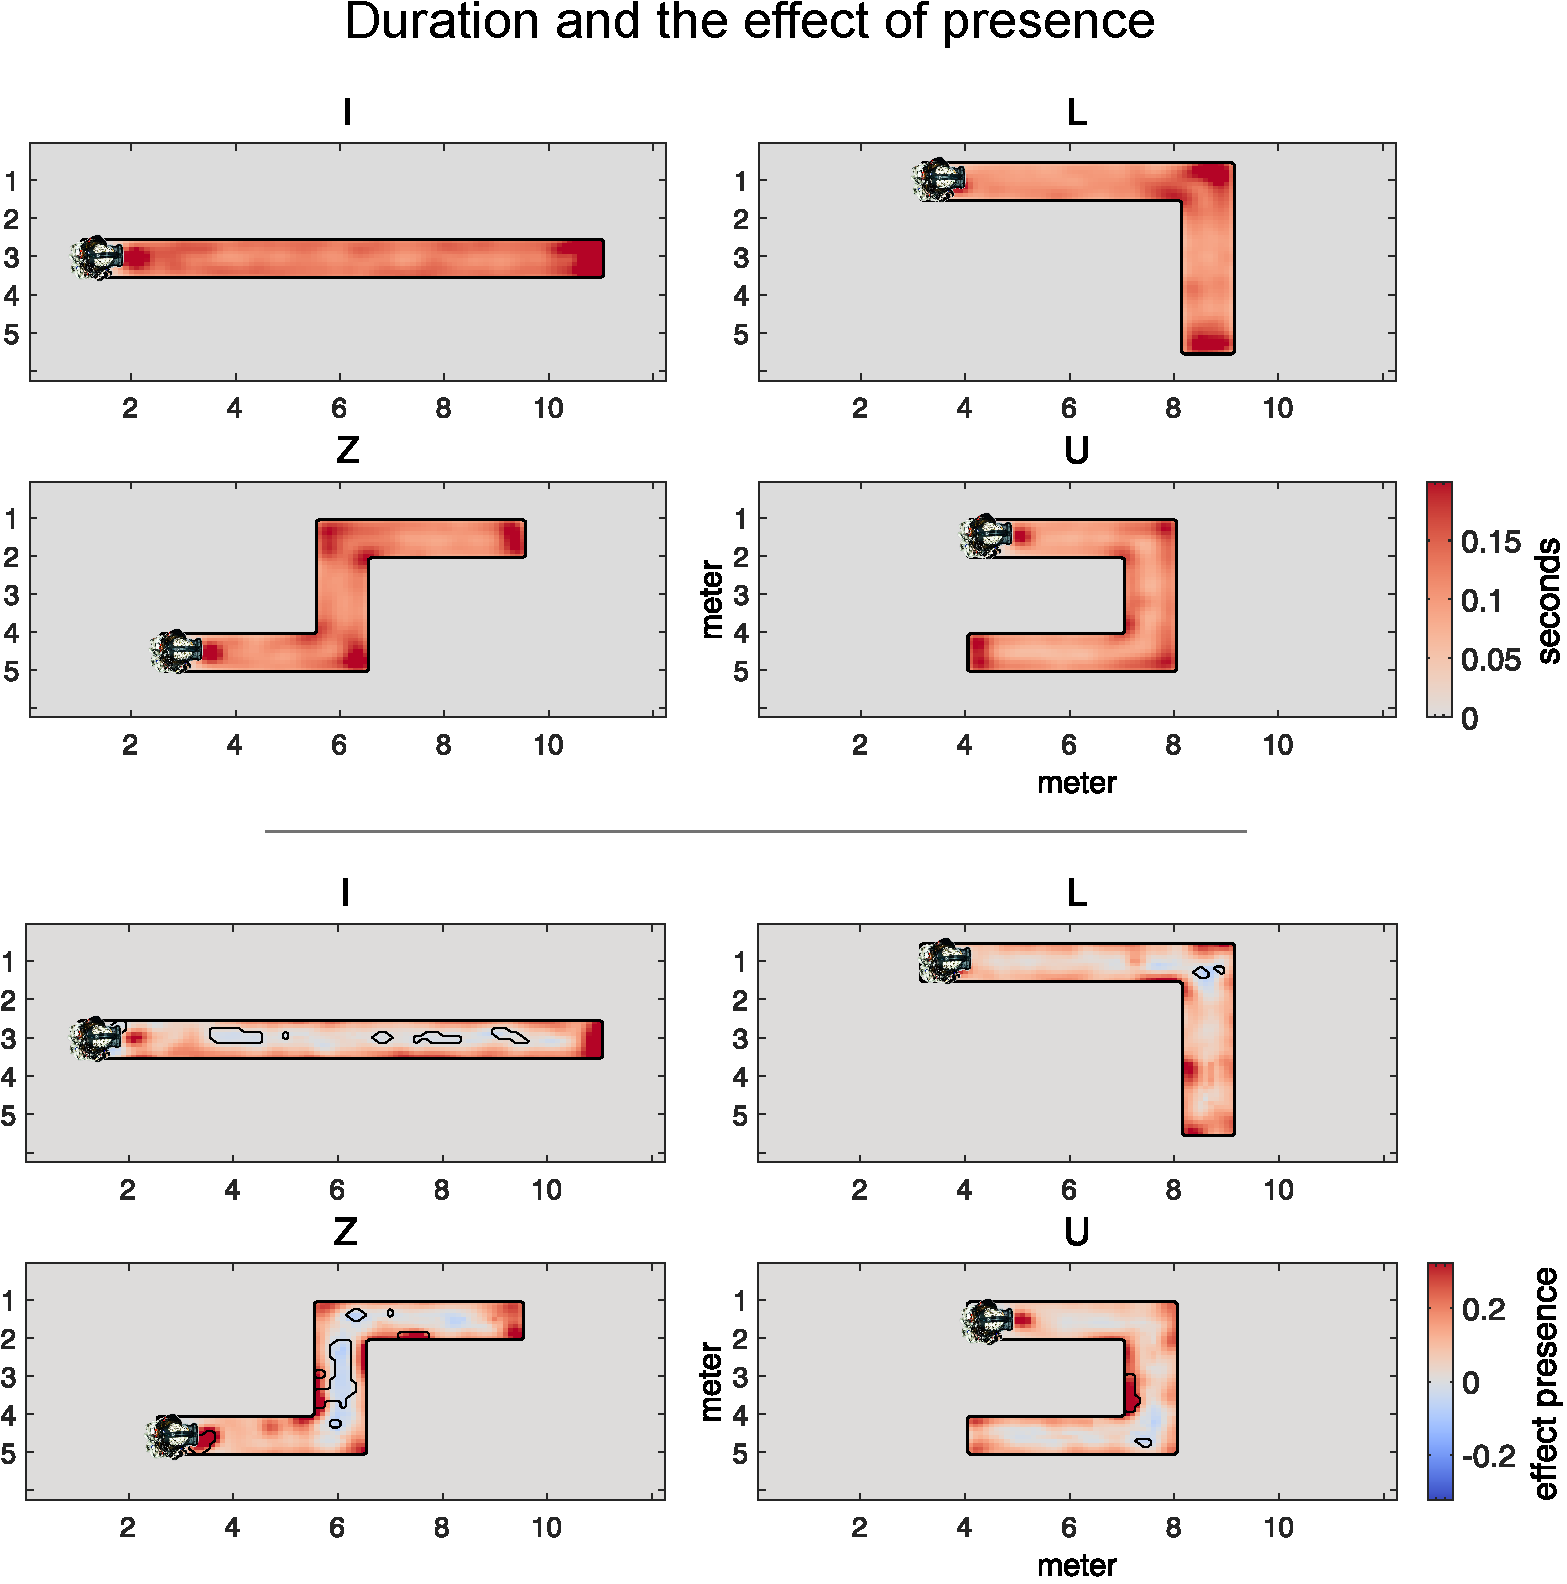
\includegraphics[width=\linewidth]{figures/duration.pdf}
\vspace{0pt}
\caption{Grand average duration in seconds spent at each location in each of the four different mazes: I, L, Z and U. The whole lab space is roughly 12 by 8 meters in size. Hotter colors, i.e. red, indicate a longer time spent at that location. Map of the impact of presence on the time spent at every location in each of the four mazes: I, L, Z, U. Warmer colors refer to a positive regression estimate. For easy readability we introduce the reasoning for a positive estimate: for each 1 point increase in reported presence, participants stayed z seconds longer at location xy.}
\label{results_duration}
\end{figure}

\subsection{Zooming in: Participants Exploration Behavior differs as a Function of Presence} First, we took a look at the grand average across participants for the two spatially resolved parameters 'time spent' as well as 'number of touches'. We observe a longer time spent at dead-ends as well as in the corners congruently across all mazes. On average participants spent about 4 second in each of hottest, i.e. reddest, locations in the corners and dead-ends, see figure \ref{results_duration}. Participants spent less time when located in the straight segments of each maze, i.e. they moved faster in those segments. For the number of touches we observed a similar pattern, see figure \ref{results_touches}. On average, participants touched the wall more frequent when located in the dead-ends and corners of the maze and exhihit less frequent wall touching along the straight segments. On average each pixel in the corners shows a likelihood of .08 that a wall was touched here.

\begin{figure}[h]
\centering
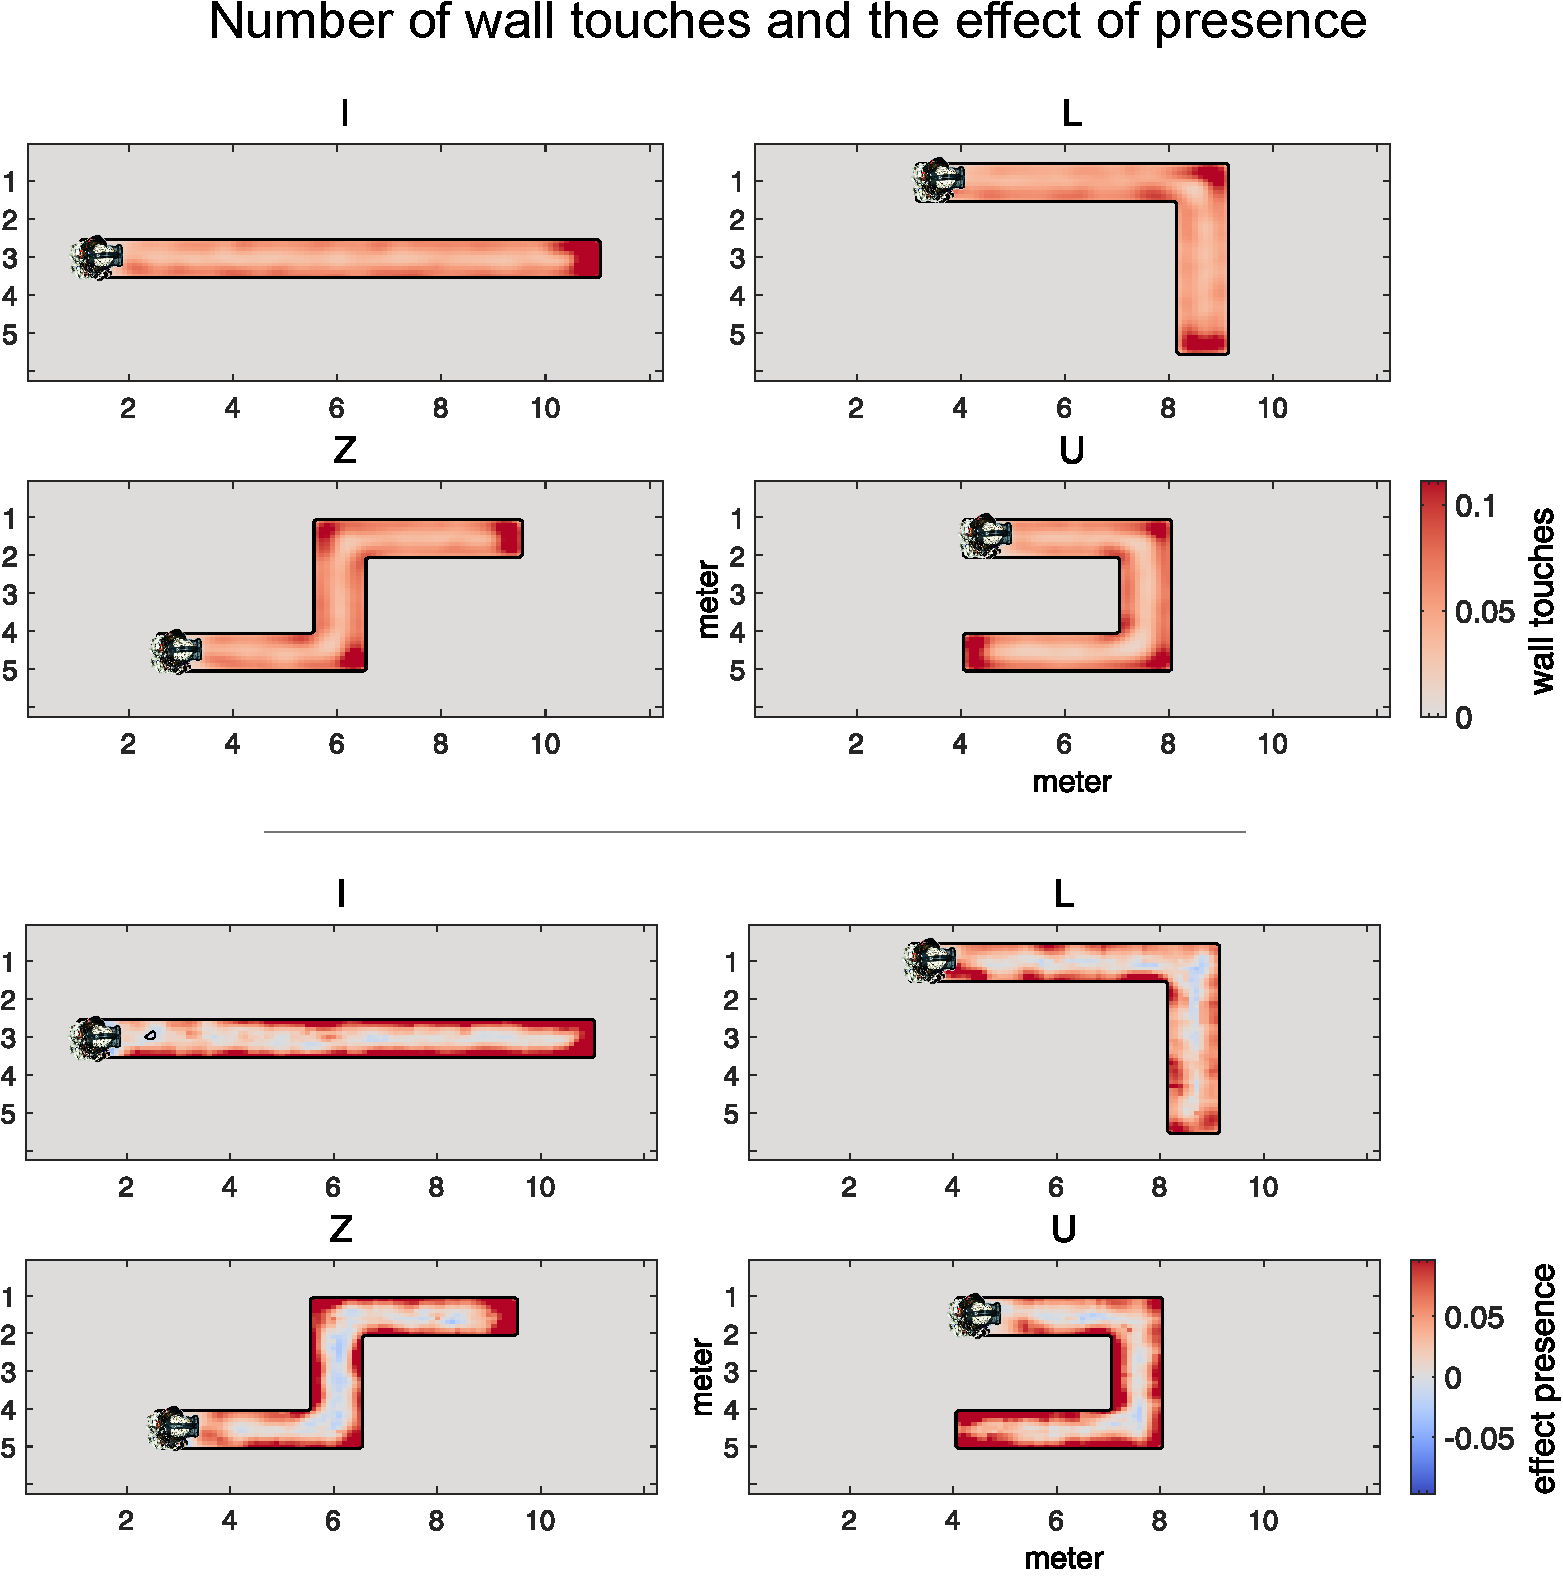
\includegraphics[width=\linewidth]{figures/touches.pdf}
\vspace{0pt}
\caption{Grand average number of touches at each location in each of the four mazes: I, L, Z, U. Hotter colors, i.e. redder, indicate a higher number of touches. Note, the location of each wall touch was located to where the participants head (VR Headset) was located at that time point, not its hand. Map of the impact of presence on the number of touches at every location in each of the four mazes: I, L, Z, U. Warmer colors refer to a positive regression estimate. For easy readability we introduce the reasoning for a positive estimate: for each 1 point increase in reported presence, participants touched the walls z times at location xy.}
\label{results_touches}
\end{figure}

Second, we investigated the effect of presence on time spent and number of touches at every location in all mazes. With increasing presence, we observed an increase in time spent at the corners and dead-ends of the mazes, see figure \ref{results_duration}. Furthermore, with increasing presence a decrease in time spent at the center of the path, the paths were 1m wide, was observed for all mazes. Interestingly, this effect was significant for portions of the straight 'I' maze as well as the second straight segment of the 'Z' maze. For the 'L' maze we observed a significant effect of presence on the time spent in the center of the first turn. Similar significant locations were observed in the second turn of the 'U' maze. Taken together, with an increase in experienced presence, participants spent more time closer to the walls and less in the center of the paths. Additionally, this effect showed most prominent in the corners of the 'L', 'Z' and 'U' maze as well as along the straight of the 'I' and 'Z' maze.

The effect of presence on the number of spatially resolved wall touches showed less spatial specificity. Participants with higher reported presence had overall more wall touches than participants with a lower score. Presence did not significantly impact the spatial distribution of wall touches during exploration. We did observe a positive effect of presence on the number of wall touches along inside corner and dead-ends of mazes 'L' and 'U'. Higher experienced presence coincided with an increase in the number of touches along those corners and dead-ends, see figure \ref{results_touches}.
\subsection{Video Game Experience, Gender and Perspective Taking predict experienced Presence} Running a step-wise model selection resulted in three predictors being kept, explaining 53,4\% of the variation in experienced presence ($F_{(3,25)}=11.69, p < .001,$ adjusted $R^2=.534$). Participants' predicted presence was equal to $8.15 - 1.2 (Video Game Experience) + 2.61 (SEX) - 0.02 (PTSOT)$ where sex was dummy-coded as 1 = Male, 2 = Female, increasing video game experience was coded with higher scores and decreasing perspective taking ability with higher scores. Video game experience ($t_{(25)}=-4.7, p<.001$), sex ($t_{(25)}=5.6, p<.001$) as well as perspective taking ability ($t_{(25)}=-2.52, p<.05$) were significant predictors of presence.
Training the three predictor model above for each of five different folds of the data and evaluating its performance on the held-out fold yielded a combined average .76 mean absolute error. Hence, using video game experience, sex as well as perspective taking ability we were able to predict experienced presence to within three-quarters of a point accuracy.

\section{Discussion}
Our work reports two relevant contributions. First it confirms established results regarding contributing factors to participants propensity to report high or low presence score after a virtual reality experience.

Besides an interest in predicting the level of experienced presence in real-time with neurophysiological metrics, investigating whether there are observable effect in overt behavior is of equal interest and importance to the ecological validity argument.

% cite results where sex and video game experience contribute to presence

presence and accuracy of motor behavior, problem because non-continuous metric, cite myself, moderated by learning/difficulty, clustering approaches

presence is best predicted by video game experience and sex (there is evidence of sex and videogame influence in slater work etc.). Interestingly, in our experiment video game experience negatively impacts presence reported on the general item of the IPQ. This may be due to the overly simplistic visuals of the virtual world. Participants with significant video gaming experience might perceive the world as too artificial.

explore exit interviews and use in discussion!

%\subsection{Disentangling Presence}
Sense of ownership, sense of agency etc.

% put first image of heatmaps of location and then hint at using mass-univariate regression on each point to increase the resolution of the investigative lens
\subsection{Challenges and Limitations}

say that behavioral metrics not informative enough in terms of presence with broad resolution, and that a finer resolution is beneficial.

Here, we addressed a potential link between presence and accuracy of motor behavior on broad scale, i.e. in an unconstrained navigation paradigm. 

Complexity of presence as a psychological construct and that it may interact with spatial learning and task difficulty among other things~\cite{} % gonzales-castro model

Increasing the resolution of the investigation to finely resolved analysis in space. Motion capture allows us to do that. 
statistics can be extended to using resampling methods, see pernet limo, spm etc.
\subsubsection{Assessing presence objectively and continuously}
The problem that we do assess it using non-continuous metrics with a time delay of administration~\cite{Gehrke:2019:DVM:3290605.3300657}. why it is interesting to look at objective predictors of presence experience?

% what to cite:
One way is through observing predictors in overt behavior, another way allowing to detect experienced presence is to go directly to the source of the signal, i.e. the brain \cite{Gehrke:2019:DVM:3290605.3300657}.
% add a sentence or two about the paper and similar work it cited, building interfaces that are 'neuroaware' and adapt their behavior based on closed-loop feedback from the brain.

% extra
% \input{chapters/credits.tex}

% Submissions are not required to reflect the precise reference formatting of the journal (use of italics, bold etc.), however it is important that all key elements of each reference are included.
\bibliography{bibliography}

\end{document}
